\subsection{Breguet Optimizer Trade Study}
The discrete Breguet optimizer swept fuel type, engine count, and specific impulse for the fixed-geometry baseline ($V=250.0\,\mathrm{m^3}$, $L/D=5.8197$, and $T_\mathrm{req}=468,393.5\,\mathrm{N}$). The sweep covered 744 total combinations with a fuel-volume cap of 15\%, a thrust margin of 1.20, and a per-engine thrust limit of 60,000\,\mathrm{N}.

Out of these 744 combinations, 20 cases (2.7\%) were feasible. The viable set was limited to JP-7 under the current mission and geometry assumptions.

\begin{figure}[htbp]
    \centering
    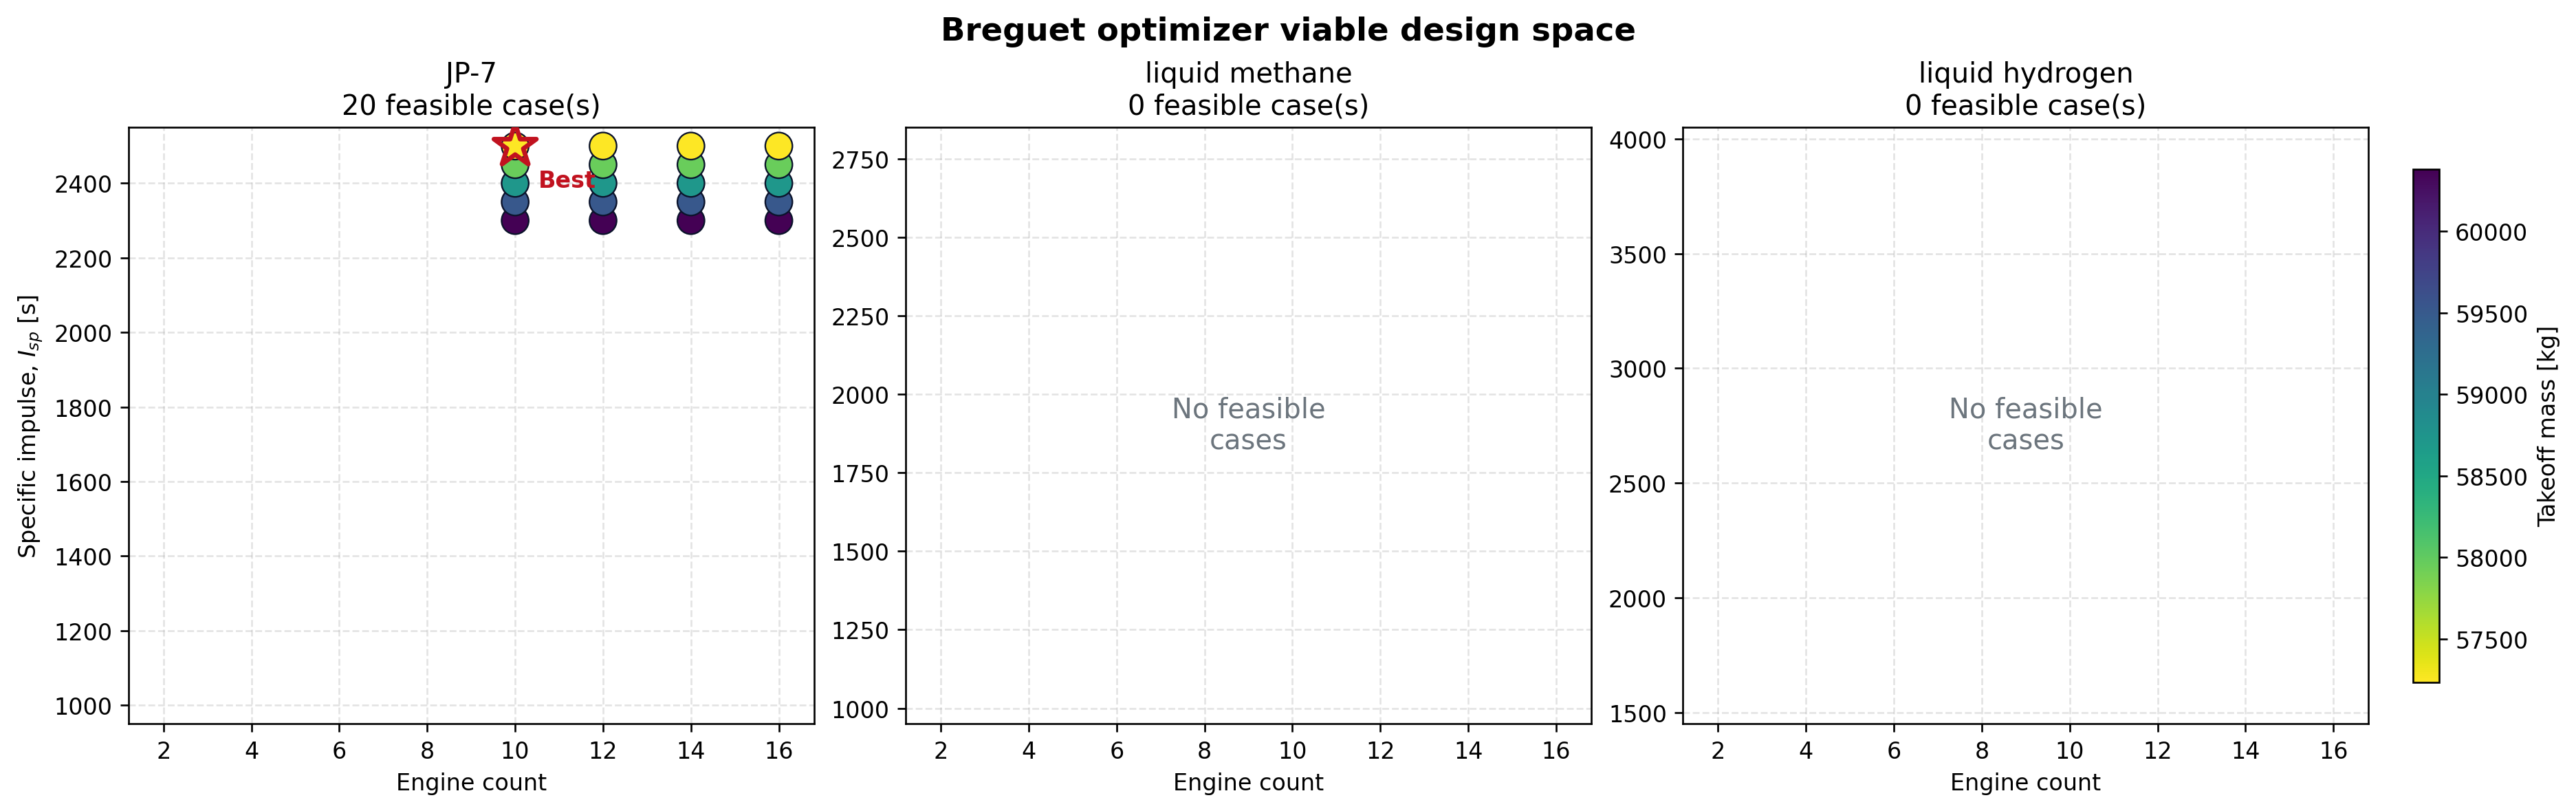
\includegraphics[width=0.98\linewidth]{runs/breguet-optimizer/viable-options.png}
    \caption{Viable Breguet optimizer cases by fuel option. Marker color denotes takeoff mass, and the red star marks the minimum-mass feasible case.}
    \label{fig:breguet-optimizer-viable-options}
\end{figure}

\begin{table}[htbp]
    \centering
    \caption{Unique viable Breguet optimizer options for the baseline configuration.}
    \begin{tabular}{lcccc}
        \hline
        Fuel & $I_{sp}$ [s] & Feasible engine counts & Fuel volume fraction & Takeoff mass [kg] \\
        \hline
        JP-7 & 2300 & 10, 12, 14, 16 & 14.67\% & 60,381.9 \\
        JP-7 & 2350 & 10, 12, 14, 16 & 14.24\% & 59,528.6 \\
        JP-7 & 2400 & 10, 12, 14, 16 & 13.84\% & 58,722.2 \\
        JP-7 & 2450 & 10, 12, 14, 16 & 13.46\% & 57,959.0 \\
        JP-7 & 2500 & 10, 12, 14, 16 & 13.10\% & 57,235.7 \\
        \hline
    \end{tabular}
    \label{tab:breguet-optimizer-viable-options}
\end{table}

The minimum-mass feasible case used JP-7 with $I_{sp}=2500\,\mathrm{s}$ and 10 engines. This case required 32.8\,\mathrm{m^3} of fuel (13.10\% of vehicle volume) and produced a takeoff mass of 57,235.7\,\mathrm{kg}.

Because the current engine-sizing model keeps total installed powerplant mass fixed for a fixed thrust requirement and thrust-to-weight ratio, engine count affects feasibility through per-engine thrust capacity but does not change takeoff mass once the thrust constraint is met. As a result, the first feasible engine count (10) is also tied with all larger feasible engine counts at the same specific impulse.

Within the feasible design space, increasing specific impulse monotonically reduced both fuel-volume fraction and takeoff mass. This indicates that propulsion efficiency, rather than additional engine multiplicity, is the dominant lever in the present Breguet-based trade study.
